
\section{Ejercicio 02}
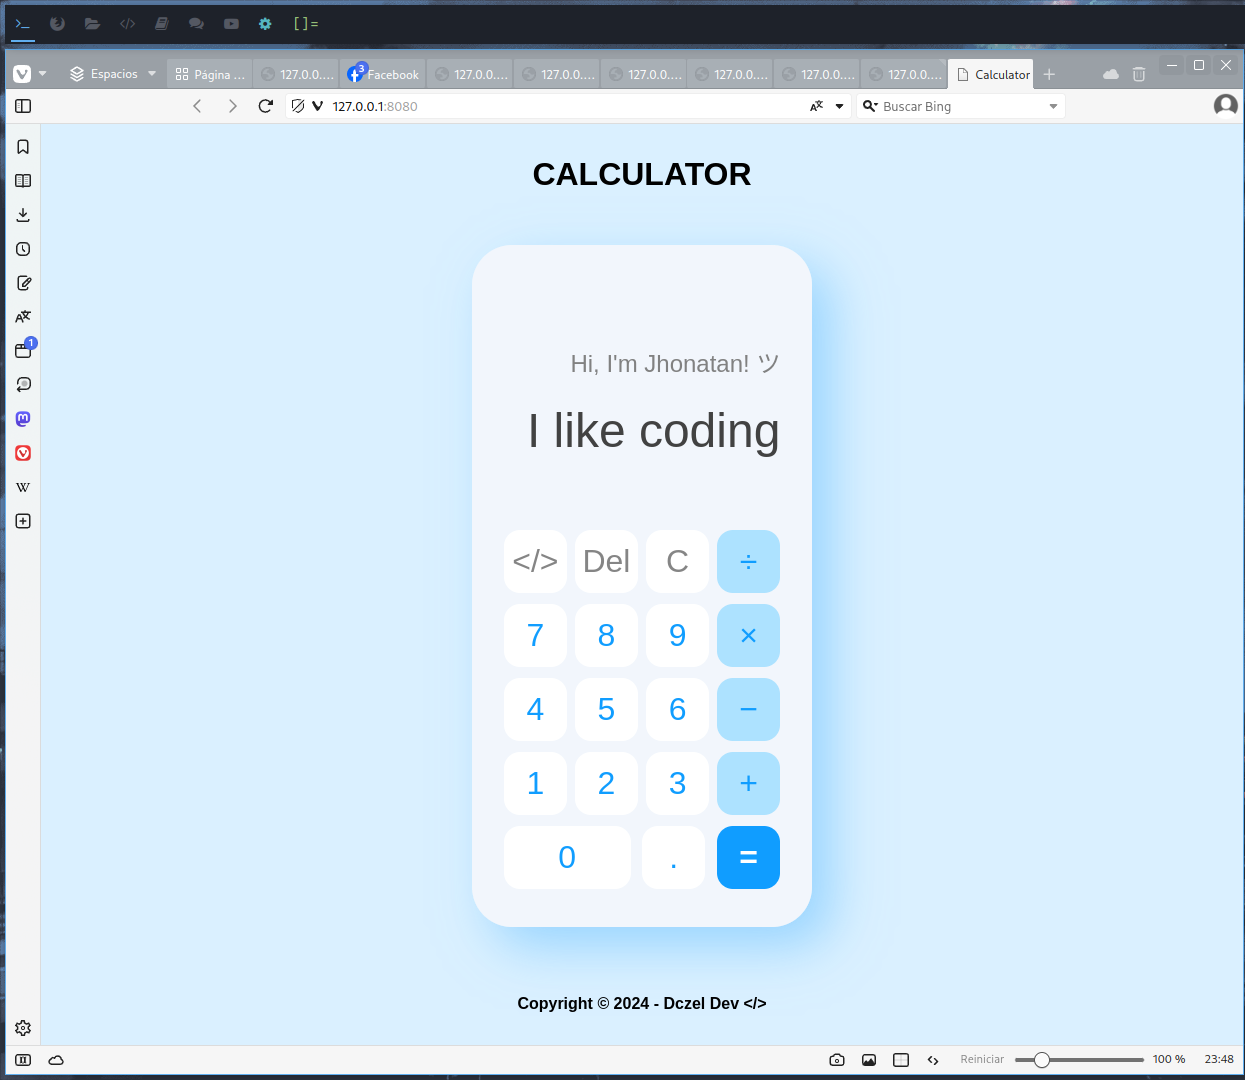
\includegraphics[width=1\textwidth]{./img/ejercicio02.png}
El archivo components contiene la estructura de html que tiene el proyecto, se aprovecha el uso de template literals para manejar mejor las cosas.
\begin{lstlisting}[language=JavaScript, caption={Archivo components.js}]

document.body.innerHTML = /*html*/`
    <div class="header">
      <h1>CALCULATOR</h1>
    </div>
    <div class="calculator">
      <div class="display">
        <div id='d1' class="display-1"></div>
        <div id='d2' class="display-2">0</div>
      </div>
      <div class="buttons">
      </div>
    </div>
    <div class="footer">
      <div class="footer">
        <a href='https://github.com/JhonatanDczel' target='_blank'><p class="autor">Copyright © 2023 - Dczel Dev <span class="icon">&lt;/&gt;</span></p></a>
      </div>
    </div>
`;
\end{lstlisting}

% Archivo easteregg.js
Es un pequeno easteregg que agregué para cuando alguien aprete el boton de </>
\begin{lstlisting}[language=JavaScript, caption={Archivo easteregg.js}]
const btn1 = document.getElementById("</>");
const btn2 = document.getElementById("2");
const btn3 = document.getElementById("0");
const btn4 = document.getElementById("6");
const d1 = document.getElementById("d1");
const d2 = document.getElementById("d2");

let event1 = false;
let event2 = false;
let event3 = false;
let event4 = false;
let time = 3000;

let desactivar = (ev) => {
  setTimeout(() => {
    ev = false;
    console.log("desactivado");
  }, time);
};

btn1.addEventListener("click", () => {
  event1 = true;
  console.log("Actived");
  desactivar(event1);
});

btn2.addEventListener("click", () => {
  event2 = true;
  console.log("Actived");
  desactivar(event2);
});

btn3.addEventListener("click", () => {
  event3 = true;
  console.log("Actived");
  desactivar(event3);
});

btn4.addEventListener("click", () => {
  event4 = true;
  console.log("Actived");
  if (event1 && event2 && event3 && event4) {
    d1.textContent = "Easter egg xd";
    d2.textContent = "No se que poner";
  }
  desactivar(event4);
});
\end{lstlisting}

% Archivo script3.js
El archivo Script3.js contiene la lógica que hace funcionar la calculadora
\begin{lstlisting}[language=JavaScript, caption={Archivo script3.js}]
//Variables globales
const buttons = document.querySelector(".buttons");

// Arreglos de botones para la interfaz
const toolBar = ["</>", "Del", "C"];
const numPad = ["7", "8", "9", "4", "5", "6", "1", "2", "3", "0", "."];
const operations = ["÷", "×", "−", "+", "="];

// Función para crear los botones de la calculadora
makeButtons();
window.addEventListener("resize", makeButtons);
\end{lstlisting}

